\documentclass[8pt,aspectratio=169]{beamer}
\usepackage[utf8]{inputenc}
\usepackage{graphicx}
\usepackage{amsmath,amssymb}
\usepackage{algorithm2e}
\usepackage{listings}
\usepackage{xcolor}
\usepackage{tikz}
\usepackage{pgfplots}
\pgfplotsset{compat=1.17}
\usepackage{subfigure}
\usepackage{hyperref}
\usepackage{multicol}
\usepackage{tcolorbox}
\usepackage{booktabs}
\usepackage{adjustbox}

% Theme settings
\usetheme{Frankfurt}
\usecolortheme{seahorse}
\setbeamertemplate{navigation symbols}{}
\setbeamertemplate{footline}[frame number]

% Custom colors
\definecolor{darkblue}{RGB}{0,51,102}
\definecolor{lightblue}{RGB}{173,216,230}
\definecolor{codegreen}{RGB}{0,128,0}
\definecolor{codegray}{RGB}{150,150,150}
\definecolor{codepurple}{RGB}{128,0,128}
\definecolor{backcolor}{RGB}{245,245,245}
\definecolor{correctgreen}{RGB}{0,150,0}
\definecolor{incorrectred}{RGB}{200,0,0}

% Code listing settings
\lstset{
    backgroundcolor=\color{backcolor},
    basicstyle=\ttfamily\footnotesize,
    breakatwhitespace=false,
    breaklines=true,
    captionpos=b,
    commentstyle=\color{codegreen},
    keywordstyle=\color{blue},
    numberstyle=\tiny\color{codegray},
    stringstyle=\color{codepurple},
    showstringspaces=false,
    frame=single,
    numbers=left,
    language=Python
}

% Custom commands (some may be defined in slide_layouts.tex)
% \newcommand{\highlight}[1]{\textcolor{blue}{\textbf{#1}}} % Already in slide_layouts
% \newcommand{\eqbox}[1]{\colorbox{yellow!20}{$\displaystyle #1$}} % Already in slide_layouts
% \newcommand{\given}{\mid} % Already in slide_layouts
% \newcommand{\prob}[1]{P(#1)} % Already in slide_layouts
% \newcommand{\argmax}{\mathrm{argmax}} % Already in slide_layouts
% \newcommand{\softmax}{\mathrm{softmax}} % Already in slide_layouts

% Include slide layouts
% SLIDE LAYOUT TEMPLATES FOR NLP COURSE
% Three consistent layouts used throughout the course

% ==============================================================
% LAYOUT 1: CONCEPT SLIDE
% Used for: Theory, definitions, mathematical concepts
% Features: Title, main content area with bullets/equations, optional figure
% ==============================================================

\newcommand{\conceptslide}[3]{ % #1: title, #2: content, #3: optional figure
\begin{frame}[t]{#1}
    \begin{columns}[T]
        \begin{column}{0.6\textwidth}
            #2
        \end{column}
        \begin{column}{0.35\textwidth}
            \centering
            #3
        \end{column}
    \end{columns}
\end{frame}
}

% ==============================================================
% LAYOUT 2: CODE & IMPLEMENTATION SLIDE
% Used for: Code examples, algorithms, implementation details
% Features: Title, code block, explanation text
% ==============================================================

% Note: For code slides, use \begin{frame}[fragile] manually

\newcommand{\codeexplanation}[1]{%
    \vspace{0.5em}
    \small
    #1
}

\newcommand{\codeblock}[2][Python]{%
    \begin{lstlisting}[language=#1, basicstyle=\ttfamily\tiny]
#2
    \end{lstlisting}
}

\newcommand{\codeslide}[3]{%
    \begin{frame}[fragile]{#1}
    \begin{columns}[T]
        \column{0.55\textwidth}
        \codeblock{#2}
        \column{0.43\textwidth}
        \codeexplanation{#3}
    \end{columns}
    \end{frame}
}

% ==============================================================
% LAYOUT 3: RESULTS & VISUALIZATION SLIDE
% Used for: Experimental results, charts, comparisons
% Features: Title, large visualization area, key insights
% ==============================================================

\newcommand{\resultslide}[3]{ % #1: title, #2: visualization, #3: insights
\begin{frame}[t]{#1}
    \centering
    \vspace{-0.5em}
    #2
    \vspace{0.5em}
    
    \begin{block}{Key Insights}
        #3
    \end{block}
\end{frame}
}

% Additional utility commands for consistency

% Highlighted text
\newcommand{\highlight}[1]{\textcolor{blue}{\textbf{#1}}}

% Math notation shortcuts
\newcommand{\prob}[1]{P(#1)}
\newcommand{\given}{\mid}
\newcommand{\argmax}{\operatorname{argmax}}
\newcommand{\softmax}{\operatorname{softmax}}

% Standard figure size
\newcommand{\stdfigsizeinchins}{0.4\textwidth}

% For code blocks, use lstlisting directly:
% \begin{lstlisting}[language=Python]
% ... code ...
% \end{lstlisting}

% Equation highlight box
\newcommand{\eqbox}[1]{
    \begin{center}
    \colorbox{lightblue!20}{
        \parbox{0.8\textwidth}{
            \vspace{0.3em}
            \centering
            #1
            \vspace{0.3em}
        }
    }
    \end{center}
}

\title[Week 2: Neural LM]{Natural Language Processing Course}
\subtitle{Week 2: Neural Language Models and Word Embeddings}
\author{Restructured with 4-Part Format}
\date{2024}

\begin{document}

% Title page
\begin{frame}
    \titlepage
\end{frame}

%============================================================================
% EVOLUTION OF LANGUAGE MODELING - MOVED TO FRONT
%============================================================================

\begin{frame}[t]{The Evolution of Language Modeling: Overview}
    \centering
    \includegraphics[width=0.9\textwidth]{../figures/week2_evolution_timeline.pdf}
    
    \vspace{0.5em}
    \textbf{Four Major Eras in Next-Word Prediction:}
    \begin{itemize}
        \item \textbf{1980s-2000s:} Statistical N-grams
        \item \textbf{2003-2013:} Neural Language Models
        \item \textbf{2013-2017:} Word Embeddings Era
        \item \textbf{2017-Present:} Transformer Revolution
    \end{itemize}
\end{frame}

\begin{frame}[t]{N-grams Era (1980s-2000s): Count and Predict}
    \textbf{How it predicted the next word:}
    
    \vspace{0.5em}
    \begin{columns}[T]
        \begin{column}{0.5\textwidth}
            \textbf{Vocabulary:}
            \begin{itemize}
                \item Fixed word list (10k-100k words)
                \item Out-of-vocabulary (OOV) → $<$UNK$>$
                \item Simple tokenization (spaces, punctuation)
            \end{itemize}
            
            \vspace{0.5em}
            \textbf{Context:}
            \begin{itemize}
                \item Fixed window (typically 2-5 words)
                \item "The cat sat" → predict next word
                \item No long-range dependencies
            \end{itemize}
        \end{column}
        \begin{column}{0.5\textwidth}
            \textbf{Method:}
            \begin{itemize}
                \item Count n-gram frequencies
                \item Markov assumption
                \item Smoothing techniques (Laplace, Kneser-Ney)
            \end{itemize}
            
            \vspace{0.5em}
            \textbf{Prediction Formula:}
            $$P(w_n|w_{n-2}, w_{n-1}) = \frac{C(w_{n-2}, w_{n-1}, w_n)}{C(w_{n-2}, w_{n-1})}$$
            
            Example: P(mat|cat, sat) = 45/50 = 0.9
        \end{column}
    \end{columns}
    
    \vspace{0.5em}
    \highlight{Strengths:} Simple, interpretable, no training needed
    
    \highlight{Limitations:} Sparsity, no semantics, fixed context
\end{frame}

% Overview
\begin{frame}[t]{Week 2: Neural Language Models - Overview}
    \begin{columns}[T]
        \begin{column}{0.48\textwidth}
            \textbf{Part 1: Introduction \& Motivation}
            \begin{itemize}
                \item Interactive word association
                \item The semantic understanding problem
                \item Real-world impact and applications
                \item Historical journey to Word2Vec
            \end{itemize}
            
            \vspace{0.5em}
            \textbf{Part 2: Core Concepts}
            \begin{itemize}
                \item Distributional hypothesis
                \item From discrete to continuous
                \item Word2Vec architecture
                \item Implementation deep dive
            \end{itemize}
        \end{column}
        \begin{column}{0.48\textwidth}
            \textbf{Part 3: Challenges \& Solutions}
            \begin{itemize}
                \item Training at scale
                \item Evaluation methodologies
                \item Fundamental limitations
                \item Advanced techniques
            \end{itemize}
            
            \vspace{0.5em}
            \textbf{Part 4: Applications \& Future}
            \begin{itemize}
                \item Hands-on applications
                \item Modern evolution (BERT, GPT)
                \item Industry state-of-the-art
                \item Looking forward
            \end{itemize}
        \end{column}
    \end{columns}
    
    \vspace{0.5em}
    \begin{center}
    \colorbox{lightblue!30}{
        \parbox{0.8\textwidth}{
            \centering
            \textbf{Goal:} Master how computers learn word meaning through context
        }
    }
    \end{center}
\end{frame}

%============================================================================
\section{Part 1: Introduction and Motivation}
%============================================================================

% Part 1 Title Slide
\begin{frame}
    \centering
    \vspace{2cm}
    {\Large \textbf{Part 1}}\\
    \vspace{0.5cm}
    {\huge \textbf{Introduction and Motivation}}\\
    \vspace{1cm}
    {\large Why Computers Need to Understand Word Meaning}
\end{frame}

% Interactive Hook
\begin{frame}[t]{Interactive Exercise: Word Association Game}
    \centering
    {\Large When you see this word, what comes to mind?}
    
    \vspace{1cm}
    {\Huge \textbf{OCEAN}}
    
    \vspace{1cm}
    \pause
    
    \begin{columns}[T]
        \begin{column}{0.25\textwidth}
            \centering
            \textcolor{correctgreen}{\textbf{water}} \\
            35\% of you
        \end{column}
        \begin{column}{0.25\textwidth}
            \centering
            \textcolor{correctgreen}{\textbf{sea}} \\
            25\% of you
        \end{column}
        \begin{column}{0.25\textwidth}
            \centering
            \textcolor{correctgreen}{\textbf{beach}} \\
            20\% of you
        \end{column}
        \begin{column}{0.25\textwidth}
            \centering
            \textcolor{correctgreen}{\textbf{waves}} \\
            20\% of you
        \end{column}
    \end{columns}
    
    \vspace{1cm}
    \highlight{You naturally understand semantic relationships!}
    
    \vspace{0.5em}
    \textbf{But until 2003, computers saw:}
    \begin{itemize}
        \item ocean = ID 7849
        \item water = ID 2341  
        \item No connection whatsoever!
    \end{itemize}
\end{frame}

% The Problem
\begin{frame}[t]{The Semantic Gap: Computers vs Humans}
    \begin{columns}[T]
        \begin{column}{0.48\textwidth}
            \textbf{How Humans See Words:}
            \begin{itemize}
                \item cat $\approx$ kitten (similar animals)
                \item Paris $\leftrightarrow$ France (location relation)
                \item running $\sim$ ran (same verb, different tense)
                \item doctor $\leftrightarrow$ hospital (association)
            \end{itemize}
            
            \vspace{0.5em}
            \colorbox{green!20}{
                \parbox{\textwidth}{
                    Rich semantic network with relationships, similarities, and associations
                }
            }
        \end{column}
        \begin{column}{0.48\textwidth}
            \textbf{How Computers Saw Words (Pre-2003):}
            \begin{itemize}
                \item cat = 1247
                \item kitten = 8923
                \item Paris = 4567
                \item France = 2109
            \end{itemize}
            
            \vspace{0.5em}
            \colorbox{red!20}{
                \parbox{\textwidth}{
                    Arbitrary IDs with no notion of meaning or relationships
                }
            }
        \end{column}
    \end{columns}
    
    \vspace{1em}
    \begin{center}
        \highlight{The Challenge: Bridge this semantic gap!}
    \end{center}
\end{frame}

% Real Failures
\begin{frame}[t]{Real System Failures Without Semantic Understanding}
    \textbf{Early Google Search (2000):}
    \begin{itemize}
        \item Search: "car" → Missed: "automobile", "vehicle"
        \item Search: "running shoes" → Missed: "jogging sneakers"
    \end{itemize}
    
    \vspace{0.5em}
    \textbf{Machine Translation Disasters:}
    \begin{itemize}
        \item "The spirit is willing but the flesh is weak" 
        \item → Russian → English: 
        \item "The vodka is good but the meat is rotten"
    \end{itemize}
    
    \vspace{0.5em}
    \textbf{Customer Service Chatbots (2005):}
    \begin{itemize}
        \item Customer: "I want to return my purchase"
        \item Bot: "I don't understand. Did you mean 'buy'?"
        \item → Couldn't link "return" with "refund", "exchange"
    \end{itemize}
    
    \vspace{0.5em}
    \begin{center}
    \colorbox{yellow!20}{
        \parbox{0.8\textwidth}{
            \centering
            \textbf{Economic Impact:} Billions lost due to poor search and translation
        }
    }
    \end{center}
\end{frame}

% Modern Impact
\begin{frame}[t]{Where Word Embeddings Power Your Life (2024)}
    \begin{columns}[T]
        \begin{column}{0.33\textwidth}
            \textbf{Entertainment:}
            \begin{itemize}
                \item \textbf{Spotify:} 256-dim song embeddings
                \item \textbf{Netflix:} Show similarity vectors
                \item \textbf{TikTok:} Video understanding
                \item \textbf{YouTube:} Related videos
            \end{itemize}
        \end{column}
        \begin{column}{0.33\textwidth}
            \textbf{Productivity:}
            \begin{itemize}
                \item \textbf{Gmail:} Smart compose (BERT)
                \item \textbf{Grammarly:} Context awareness
                \item \textbf{Notion AI:} Semantic search
                \item \textbf{Slack:} Message threading
            \end{itemize}
        \end{column}
        \begin{column}{0.33\textwidth}
            \textbf{Commerce:}
            \begin{itemize}
                \item \textbf{Amazon:} Product similarity
                \item \textbf{Google Ads:} Ad matching
                \item \textbf{Airbnb:} Listing embeddings
                \item \textbf{Uber:} Location understanding
            \end{itemize}
        \end{column}
    \end{columns}
    
    \vspace{1em}
    \textbf{Market Size:}
    \begin{itemize}
        \item Embedding API Market: \$2.7B by 2025
        \item OpenAI Embeddings: 1M+ developers
        \item Vector Database Market: \$4.3B by 2028
    \end{itemize}
    
    \vspace{0.5em}
    \begin{center}
        \highlight{Every AI application today relies on word embeddings!}
    \end{center}
\end{frame}

% Historical Journey
\begin{frame}[t]{The Journey to Understanding: Timeline}
    \begin{center}
    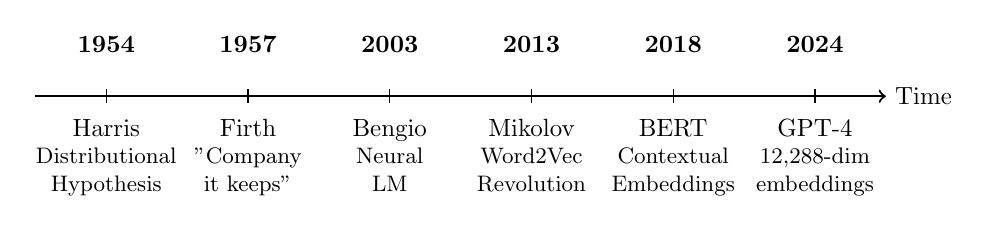
\begin{tikzpicture}[scale=0.9, transform shape]
        % Timeline
        \draw[thick,->] (0,0) -- (12,0) node[right] {Time};
        
        % Events
        \node[above] at (1,0.5) {\textbf{1954}};
        \node[below] at (1,-0.2) {Harris};
        \node[below] at (1,-0.6) {\small Distributional};
        \node[below] at (1,-1) {\small Hypothesis};
        
        \node[above] at (3,0.5) {\textbf{1957}};
        \node[below] at (3,-0.2) {Firth};
        \node[below] at (3,-0.6) {\small "Company};
        \node[below] at (3,-1) {\small it keeps"};
        
        \node[above] at (5,0.5) {\textbf{2003}};
        \node[below] at (5,-0.2) {Bengio};
        \node[below] at (5,-0.6) {\small Neural};
        \node[below] at (5,-1) {\small LM};
        
        \node[above] at (7,0.5) {\textbf{2013}};
        \node[below] at (7,-0.2) {Mikolov};
        \node[below] at (7,-0.6) {\small Word2Vec};
        \node[below] at (7,-1) {\small Revolution};
        
        \node[above] at (9,0.5) {\textbf{2018}};
        \node[below] at (9,-0.2) {BERT};
        \node[below] at (9,-0.6) {\small Contextual};
        \node[below] at (9,-1) {\small Embeddings};
        
        \node[above] at (11,0.5) {\textbf{2024}};
        \node[below] at (11,-0.2) {GPT-4};
        \node[below] at (11,-0.6) {\small 12,288-dim};
        \node[below] at (11,-1) {\small embeddings};
        
        % Marks
        \foreach \x in {1,3,5,7,9,11}
            \draw (\x,0.1) -- (\x,-0.1);
    \end{tikzpicture}
    \end{center}
    
    \vspace{1em}
    \textbf{Key Breakthroughs:}
    \begin{itemize}
        \item \textbf{1954-1957:} Theoretical foundation - words defined by context
        \item \textbf{2003:} First neural language model with continuous representations
        \item \textbf{2013:} Word2Vec makes embeddings practical and scalable
        \item \textbf{2018:} Contextualized embeddings (same word, different contexts)
        \item \textbf{2024:} Massive embeddings powering GPT-4, Claude, Gemini
    \end{itemize}
\end{frame}

% The Breakthrough
\begin{frame}[t]{The 2013 Breakthrough: King - Man + Woman = ?}
    \textbf{The demo that shocked the NLP world:}\footnotemark
    
    \vspace{0.5em}
    \begin{center}
    {\Huge king - man + woman = \pause queen}
    \end{center}
    
    \vspace{1em}
    \textbf{Why this was revolutionary:}
    \begin{itemize}
        \item Computer discovered gender relationships automatically
        \item No one programmed these rules
        \item Learned purely from reading text
        \item Worked across many relationship types
    \end{itemize}
    
    \vspace{0.5em}
    \textbf{More examples that work:}
    \begin{columns}[T]
        \begin{column}{0.48\textwidth}
            \begin{itemize}
                \item Paris - France + Italy = Rome
                \item sushi - Japan + Mexico = tacos
                \item Einstein - scientist + artist = Picasso
            \end{itemize}
        \end{column}
        \begin{column}{0.48\textwidth}
            \begin{itemize}
                \item bigger - big + small = smaller
                \item walking - walk + swim = swimming
                \item CEO - company + country = president
            \end{itemize}
        \end{column}
    \end{columns}
    
    \footnotetext{Mikolov et al. (2013). "Linguistic regularities in continuous space word representations"}
\end{frame}

% Part 1 Summary
\begin{frame}[t]{Part 1 Summary: Why This Matters}
    \textbf{Key Insights:}
    \begin{enumerate}
        \item \highlight{The Problem:} Computers treating words as meaningless IDs
        \item \highlight{The Impact:} Billions in losses, poor user experiences
        \item \highlight{The Solution:} Learn meaning from context (distributional hypothesis)
        \item \highlight{The Breakthrough:} Word2Vec made it practical (2013)
    \end{enumerate}
    
    \vspace{1em}
    \textbf{What's Next:}
    \begin{itemize}
        \item Part 2: How do we actually create these word vectors?
        \item Understanding the mathematics and algorithms
        \item Building Word2Vec from scratch
    \end{itemize}
    
    \vspace{1em}
    \begin{center}
    \colorbox{yellow!20}{
        \parbox{0.8\textwidth}{
            \centering
            \textbf{Remember:} Every modern AI system (ChatGPT, Claude, Gemini) started here!
        }
    }
    \end{center}
\end{frame}

%============================================================================
\section{Part 2: Core Concepts}
%============================================================================

% Part 2 Title Slide
\begin{frame}
    \centering
    \vspace{2cm}
    {\Large \textbf{Part 2}}\\
    \vspace{0.5cm}
    {\huge \textbf{Core Concepts}}\\
    \vspace{1cm}
    {\large How Computers Learn Word Meaning from Context}
\end{frame}

% Distributional Hypothesis
\begin{frame}[t]{The Distributional Hypothesis: Foundation}
    \textbf{Core Principle (Firth, 1957):}
    \begin{center}
    \colorbox{yellow!20}{
        \parbox{0.8\textwidth}{
            \centering
            \Large "You shall know a word by the company it keeps"
        }
    }
    \end{center}
    
    \vspace{0.5em}
    \textbf{Example: What is a "zorb"?}
    \begin{itemize}
        \item The \underline{zorb} ate the cheese
        \item I saw a \underline{zorb} in my garden
        \item The \underline{zorb} ran under the couch
        \item My cat chased the \underline{zorb}
    \end{itemize}
    
    \pause
    \highlight{You probably guessed: zorb = mouse (or similar small animal)}
    
    \vspace{0.5em}
    \textbf{Mathematical Formulation:}
    \begin{itemize}
        \item Words with similar distributions have similar meanings
        \item $\text{similarity}(w_1, w_2) \propto P(\text{context}|w_1) \cdot P(\text{context}|w_2)$
        \item Context defines meaning!
    \end{itemize}
\end{frame}

% Interactive Context Exercise
\begin{frame}[t]{Interactive: Guess the Word from Context}
    \textbf{Mystery word = [BLANK]. What is it?}
    
    \vspace{0.5em}
    \begin{enumerate}
        \item The [BLANK] was delicious
        \item I ordered [BLANK] with extra cheese
        \item The [BLANK] delivery arrived in 30 minutes
        \item We shared a large [BLANK] at the party
        \item My favorite [BLANK] topping is pepperoni
    \end{enumerate}
    
    \pause
    \vspace{0.5em}
    \highlight{Answer: pizza}
    
    \vspace{0.5em}
    \textbf{This is exactly how Word2Vec learns:}
    \begin{itemize}
        \item Sees millions of sentences
        \item Learns what words appear in similar contexts
        \item Groups them close together in vector space
        \item No dictionary needed!
    \end{itemize}
\end{frame}

% From Discrete to Continuous
\begin{frame}[t]{From Discrete IDs to Continuous Vectors}
    \begin{columns}[T]
        \begin{column}{0.48\textwidth}
            \textbf{One-Hot Encoding (Old Way):}
            \begin{itemize}
                \item Vocabulary size: 50,000 words
                \item cat = [0,0,1,0,0,...,0] (50K dimensions!)
                \item dog = [0,0,0,1,0,...,0]
            \end{itemize}
            
            \vspace{0.5em}
            \textbf{Problems:}
            \begin{itemize}
                \item \textcolor{red}{No similarity}: cat · dog = 0
                \item \textcolor{red}{Huge vectors}: 50K dimensions
                \item \textcolor{red}{Sparse}: 49,999 zeros
                \item \textcolor{red}{No learning}: Fixed representation
            \end{itemize}
        \end{column}
        \begin{column}{0.48\textwidth}
            \textbf{Dense Embeddings (Word2Vec):}
            \begin{itemize}
                \item Typical size: 100-300 dimensions
                \item cat = [0.2, -0.4, 0.7, ..., 0.1]
                \item dog = [0.3, -0.3, 0.6, ..., 0.2]
            \end{itemize}
            
            \vspace{0.5em}
            \textbf{Benefits:}
            \begin{itemize}
                \item \textcolor{green}{Similarity}: cat · dog = 0.89
                \item \textcolor{green}{Compact}: 100-300 dims
                \item \textcolor{green}{Dense}: All values meaningful
                \item \textcolor{green}{Learnable}: Updated during training
            \end{itemize}
        \end{column}
    \end{columns}
    
    \vspace{0.5em}
    \begin{center}
        \highlight{Key: Every dimension captures some semantic property}
    \end{center}
\end{frame}

% Why 100-300 Dimensions
\begin{frame}[t]{The Goldilocks Zone: Why 100-300 Dimensions?}
    \centering
    \includegraphics[width=0.7\textwidth]{../figures/embedding_dimensions_performance.pdf}
    
    \vspace{0.5em}
    \textbf{Empirical Findings:}
    \begin{itemize}
        \item \textbf{< 50 dims:} Too compressed, loses nuances
        \item \textbf{100-300 dims:} Sweet spot for most tasks
        \item \textbf{> 500 dims:} Diminishing returns, overfitting risk
    \end{itemize}
    
    \vspace{0.5em}
    \textbf{Modern Systems (2024):}
    \begin{itemize}
        \item Word2Vec: 300 dimensions
        \item OpenAI ada-002: 1,536 dimensions
        \item GPT-4 internal: 12,288 dimensions (but for full tokens, not just words)
    \end{itemize}
\end{frame}

% Word2Vec Architecture Choice
\begin{frame}[t]{Word2Vec: Two Architectures}
    \begin{columns}[T]
        \begin{column}{0.48\textwidth}
            \textbf{CBOW (Continuous Bag of Words):}
            \begin{center}
                \includegraphics[width=0.9\textwidth]{../figures/cbow_architecture.pdf}
            \end{center}
            \begin{itemize}
                \item Predict center from context
                \item Input: [the, cat, on, mat]
                \item Output: sat
                \item Faster to train
                \item Better for frequent words
            \end{itemize}
        \end{column}
        \begin{column}{0.48\textwidth}
            \textbf{Skip-gram:}
            \begin{center}
                \includegraphics[width=0.9\textwidth]{../figures/skipgram_architecture.pdf}
            \end{center}
            \begin{itemize}
                \item Predict context from center
                \item Input: sat
                \item Output: [the, cat, on, mat]
                \item Slower but more accurate
                \item Better for rare words
            \end{itemize}
        \end{column}
    \end{columns}
    
    \vspace{0.5em}
    \begin{center}
        \highlight{Skip-gram is more popular due to better performance on rare words}
    \end{center}
\end{frame}

% Skip-gram Training Example
\begin{frame}[t]{Skip-gram Training: Step by Step}
    \textbf{Sentence:} "The quick brown fox jumps"
    
    \vspace{0.5em}
    \textbf{Window size = 2} (look 2 words left and right)
    
    \vspace{0.5em}
    \begin{center}
    \begin{tabular}{|c|c|l|}
        \hline
        \textbf{Step} & \textbf{Center Word} & \textbf{Context to Predict} \\
        \hline
        1 & quick & [the, brown] \\
        2 & brown & [the, quick, fox, jumps] \\
        3 & fox & [quick, brown, jumps] \\
        \hline
    \end{tabular}
    \end{center}
    
    \vspace{0.5em}
    \textbf{Training Process:}
    \begin{enumerate}
        \item Take center word embedding
        \item Try to predict context words
        \item Measure prediction error
        \item Update embeddings to reduce error
        \item Repeat millions of times
    \end{enumerate}
    
    \vspace{0.5em}
    \highlight{Result: Words appearing in similar contexts get similar embeddings}
\end{frame}

% Implementation Code
\begin{frame}[fragile]{Implementing Word2Vec in PyTorch}
\begin{columns}[T]
\column{0.58\textwidth}
\begin{lstlisting}[language=Python, basicstyle=\ttfamily\tiny]
import torch
import torch.nn as nn
import torch.nn.functional as F

class Word2Vec(nn.Module):
    def __init__(self, vocab_size, embed_dim=100):
        super().__init__()
        # Two embedding matrices
        self.center_embeddings = nn.Embedding(
            vocab_size, embed_dim
        )
        self.context_embeddings = nn.Embedding(
            vocab_size, embed_dim
        )
        
    def forward(self, center, context, neg_samples):
        # Get embeddings
        center_emb = self.center_embeddings(center)
        context_emb = self.context_embeddings(context)
        neg_emb = self.context_embeddings(neg_samples)
        
        # Positive samples (should be similar)
        pos_score = torch.sum(
            center_emb * context_emb, dim=1
        )
        pos_loss = F.logsigmoid(pos_score)
        
        # Negative samples (should be different)
        neg_score = torch.bmm(
            neg_emb, center_emb.unsqueeze(2)
        ).squeeze()
        neg_loss = F.logsigmoid(-neg_score).sum(1)
        
        return -(pos_loss + neg_loss).mean()
\end{lstlisting}

\column{0.4\textwidth}
\textbf{Key Components:}
\begin{itemize}
    \item \textbf{Two matrices:} Center and context embeddings
    \item \textbf{Positive samples:} Real context words
    \item \textbf{Negative samples:} Random words (not in context)
\end{itemize}

\vspace{0.5em}
\textbf{Training Trick:}
\begin{itemize}
    \item Full softmax over 50K words is expensive
    \item Solution: Negative sampling
    \item Only update a few random words
    \item 5-20 negative samples typical
\end{itemize}

\vspace{0.5em}
\textbf{Loss Function:}
\begin{itemize}
    \item Maximize similarity with real context
    \item Minimize similarity with random words
\end{itemize}
\end{columns}
\end{frame}

% Training Loop
\begin{frame}[fragile]{Training Word2Vec: The Complete Loop}
\begin{lstlisting}[language=Python, basicstyle=\ttfamily\tiny]
def train_word2vec(corpus, vocab_size, embed_dim=100, epochs=5, window=2):
    model = Word2Vec(vocab_size, embed_dim)
    optimizer = torch.optim.Adam(model.parameters(), lr=0.001)
    
    for epoch in range(epochs):
        total_loss = 0
        for sentence in corpus:
            # Generate training samples from sentence
            for i, center_word in enumerate(sentence):
                # Get context words within window
                context_words = []
                for j in range(max(0, i-window), min(len(sentence), i+window+1)):
                    if i != j:
                        context_words.append(sentence[j])
                
                # Get negative samples (5 random words not in context)
                neg_samples = get_negative_samples(vocab_size, 5, avoid=context_words)
                
                # Forward pass
                loss = model(center_word, context_words, neg_samples)
                
                # Backward pass
                optimizer.zero_grad()
                loss.backward()
                optimizer.step()
                
                total_loss += loss.item()
        
        print(f"Epoch {epoch}: Loss = {total_loss:.4f}")
    
    return model.center_embeddings.weight.data  # Final embeddings
\end{lstlisting}

\textbf{Result:} After training on millions of sentences, similar words cluster together!
\end{frame}

% Visualization of Learning
\begin{frame}[t]{Visualizing What Word2Vec Learns}
    \centering
    \includegraphics[width=0.8\textwidth]{../figures/word2vec_clusters.pdf}
    
    \vspace{0.5em}
    \textbf{Automatic Clustering:}
    \begin{itemize}
        \item No one told the model about categories
        \item Learned purely from context patterns
        \item Similar contexts → nearby vectors
    \end{itemize}
\end{frame}

% Mathematical Intuition
\begin{frame}[t]{Mathematical Intuition: Why Dot Product = Similarity}
    \textbf{The Skip-gram Objective:}
    $$\max \sum_{t=1}^{T} \sum_{-c \leq j \leq c, j \neq 0} \log P(w_{t+j} | w_t)$$
    
    \vspace{0.5em}
    \textbf{Where probability is defined as:}
    $$P(w_O | w_I) = \frac{\exp(v_{w_O}^T v_{w_I})}{\sum_{w=1}^{W} \exp(v_w^T v_{w_I})}$$
    
    \vspace{0.5em}
    \textbf{Key Insight:}
    \begin{itemize}
        \item Dot product $v_{w_O}^T v_{w_I}$ measures similarity
        \item Higher dot product → higher probability of co-occurrence
        \item Training maximizes dot product for words that appear together
        \item Result: Similar words have high dot product (cosine similarity)
    \end{itemize}
    
    \vspace{0.5em}
    \begin{center}
    \colorbox{yellow!20}{
        \parbox{0.8\textwidth}{
            \centering
            Geometry emerges from statistics: Similar contexts → Similar vectors
        }
    }
    \end{center}
\end{frame}

% Part 2 Summary
\begin{frame}[t]{Part 2 Summary: Core Concepts Mastered}
    \textbf{What We Learned:}
    \begin{enumerate}
        \item \highlight{Distributional Hypothesis:} Context defines meaning
        \item \highlight{Dense Vectors:} 100-300 dimensions capture semantics
        \item \highlight{Skip-gram Model:} Predict context from center word
        \item \highlight{Training Process:} Maximize co-occurrence probability
        \item \highlight{Implementation:} Two embedding matrices + negative sampling
    \end{enumerate}
    
    \vspace{1em}
    \textbf{Key Takeaways:}
    \begin{itemize}
        \item Word meaning emerges from statistical patterns
        \item No linguistic knowledge required
        \item Scalable to millions of words
        \item Foundation for all modern NLP
    \end{itemize}
    
    \vspace{1em}
    \textbf{Next: Part 3 - Challenges and Solutions}
    \begin{itemize}
        \item How to train on billions of words efficiently?
        \item How to evaluate embedding quality?
        \item What are the limitations?
    \end{itemize}
\end{frame}

%============================================================================
\section{Part 3: Challenges and Solutions}
%============================================================================

% Part 3 Title Slide
\begin{frame}
    \centering
    \vspace{2cm}
    {\Large \textbf{Part 3}}\\
    \vspace{0.5cm}
    {\huge \textbf{Challenges and Solutions}}\\
    \vspace{1cm}
    {\large Scaling, Evaluation, and Limitations}
\end{frame}

% Softmax Visualization
\begin{frame}[t]{Softmax: From Scores to Probabilities}
    \textbf{Example: Next word prediction after "The cat sat on the..."}
    
    \vspace{0.5em}
    \begin{columns}[T]
        \begin{column}{0.45\textwidth}
            \textbf{Step 1: Neural Network Scores}
            \begin{center}
            \begin{tabular}{lr}
                \hline
                \textbf{Word} & \textbf{Score} \\
                \hline
                mat & 2.1 \\
                floor & 1.8 \\
                chair & 0.3 \\
                table & 0.1 \\
                sky & -1.2 \\
                \hline
            \end{tabular}
            \end{center}
            
            \vspace{0.5em}
            \textbf{Step 2: Apply Exponential}
            \begin{center}
            \begin{tabular}{lr}
                \hline
                \textbf{Word} & \textbf{exp(score)} \\
                \hline
                mat & 8.17 \\
                floor & 6.05 \\
                chair & 1.35 \\
                table & 1.11 \\
                sky & 0.30 \\
                \hline
                \textbf{Sum} & \textbf{16.98} \\
                \hline
            \end{tabular}
            \end{center}
        \end{column}
        \begin{column}{0.45\textwidth}
            \textbf{Step 3: Normalize (Divide by Sum)}
            \begin{center}
            \begin{tabular}{lr}
                \hline
                \textbf{Word} & \textbf{Probability} \\
                \hline
                mat & 0.481 \\
                floor & 0.356 \\
                chair & 0.079 \\
                table & 0.065 \\
                sky & 0.018 \\
                \hline
                \textbf{Sum} & \textbf{1.000} \\
                \hline
            \end{tabular}
            \end{center}
            
            \vspace{0.5em}
            \colorbox{yellow!20}{\parbox{\textwidth}{
                \centering
                \textbf{Softmax Formula:}\\
                \vspace{0.2em}
                $P(w_i) = \dfrac{e^{s_i}}{\sum_j e^{s_j}}$
            }}
            
            \vspace{0.5em}
            \highlight{Result:} "mat" has 48.1\% probability!
        \end{column}
    \end{columns}
\end{frame}

\begin{frame}[t]{Softmax Function: Mathematical Behavior}
    \centering
    \includegraphics[width=0.95\textwidth]{../figures/softmax_function_plot.pdf}
    
    \vspace{0.3em}
    \textbf{Key Properties:}
    \begin{itemize}
        \item \textbf{Single variable:} Reduces to sigmoid function
        \item \textbf{Multi-class:} Competition between classes - increasing one score decreases others' probabilities
        \item \textbf{Saturation:} Extreme values lead to near 0 or 1 probabilities
    \end{itemize}
\end{frame}

\begin{frame}[t]{Temperature in Softmax: Controlling Randomness}
    \centering
    \includegraphics[width=0.9\textwidth]{../figures/softmax_temperature_effect.pdf}
    
    \vspace{0.5em}
    \textbf{Temperature Parameter:} $P(w_i) = \dfrac{e^{s_i/T}}{\sum_j e^{s_j/T}}$
    
    \begin{itemize}
        \item \textbf{Low T (0.5):} Sharp distribution → deterministic
        \item \textbf{Normal T (1.0):} Standard softmax
        \item \textbf{High T (5.0):} Uniform distribution → random
    \end{itemize}
\end{frame}

% Computational Challenges
\begin{frame}[t]{Challenge 1: Computational Complexity}
    \textbf{The Softmax Bottleneck:}
    
    Original formulation requires normalizing over entire vocabulary:
    $$P(w_O | w_I) = \frac{\exp(v_{w_O}^T v_{w_I})}{\sum_{w=1}^{W} \exp(v_w^T v_{w_I})}$$
    
    \vspace{0.5em}
    \textbf{Problem:}
    \begin{itemize}
        \item Vocabulary size W = 50,000+ words
        \item Must compute 50,000 dot products per training step
        \item Billions of training steps needed
        \item \textcolor{red}{Computationally infeasible!}
    \end{itemize}
    
    \vspace{0.5em}
    \textbf{Solutions:}
    \begin{columns}[T]
        \begin{column}{0.48\textwidth}
            \textbf{1. Hierarchical Softmax:}
            \begin{itemize}
                \item Binary tree of words
                \item $O(\log W)$ instead of $O(W)$
                \item Path through tree to each word
            \end{itemize}
        \end{column}
        \begin{column}{0.48\textwidth}
            \textbf{2. Negative Sampling:}
            \begin{itemize}
                \item Only update k random words
                \item Typically k = 5-20
                \item Dramatic speedup
                \item Better performance!
            \end{itemize}
        \end{column}
    \end{columns}
\end{frame}

% Negative Sampling Deep Dive
\begin{frame}[t]{Solution: Negative Sampling Explained}
    \textbf{Instead of:} Predicting the right word from 50,000 options
    
    \textbf{We ask:} Is this word the right context word? (Binary classification)
    
    \vspace{0.5em}
    \begin{center}
    \begin{tabular}{|l|c|c|}
        \hline
        \textbf{Center} & \textbf{Word} & \textbf{Label} \\
        \hline
        cat & sits (real context) & 1 \\
        cat & on (real context) & 1 \\
        cat & elephant (random) & 0 \\
        cat & democracy (random) & 0 \\
        cat & quantum (random) & 0 \\
        \hline
    \end{tabular}
    \end{center}
    
    \vspace{0.5em}
    \textbf{Sampling Strategy:}
    \begin{itemize}
        \item Sample negative words by frequency: $P(w) \propto f(w)^{3/4}$
        \item The 3/4 power reduces dominance of very common words
        \item Gives rare words more chance to be negative samples
    \end{itemize}
    
    \vspace{0.5em}
    \highlight{Result: 1000x speedup with better quality embeddings!}
\end{frame}

% Evaluation Challenges
\begin{frame}[t]{Challenge 2: How Do We Evaluate Embeddings?}
    \textbf{The Problem:} How do we know if our embeddings are "good"?
    
    \vspace{0.5em}
    \begin{columns}[T]
        \begin{column}{0.48\textwidth}
            \textbf{Intrinsic Evaluation:}
            \begin{itemize}
                \item \textbf{Word Similarity:}
                    \begin{itemize}
                        \item Dataset: WordSim-353
                        \item Human ratings vs cosine similarity
                        \item Correlation: 0.6-0.7 typical
                    \end{itemize}
                \item \textbf{Word Analogies:}
                    \begin{itemize}
                        \item king - man + woman = ?
                        \item Google analogy dataset
                        \item Accuracy: 60-75\% typical
                    \end{itemize}
            \end{itemize}
        \end{column}
        \begin{column}{0.48\textwidth}
            \textbf{Extrinsic Evaluation:}
            \begin{itemize}
                \item \textbf{Downstream Tasks:}
                    \begin{itemize}
                        \item Sentiment analysis
                        \item Named entity recognition
                        \item Machine translation
                    \end{itemize}
                \item \textbf{Key Finding:}
                    \begin{itemize}
                        \item Good intrinsic $\neq$ Good extrinsic
                        \item Task-specific fine-tuning helps
                    \end{itemize}
            \end{itemize}
        \end{column}
    \end{columns}
    
    \vspace{1em}
    \textbf{Modern Approach (2024):}
    \begin{itemize}
        \item Skip intrinsic evaluation
        \item Directly evaluate on downstream tasks
        \item Use pre-trained embeddings as starting point
    \end{itemize}
\end{frame}

% Polysemy Problem
\begin{frame}[t]{Challenge 3: The Polysemy Problem}
    \textbf{One Vector Per Word... But Words Have Multiple Meanings!}
    
    \vspace{0.5em}
    \textbf{Example: "bank"}
    \begin{itemize}
        \item "I deposited money at the \textcolor{blue}{bank}" (financial institution)
        \item "We sat by the river \textcolor{red}{bank}" (edge of river)
    \end{itemize}
    
    \vspace{0.5em}
    \textbf{Word2Vec gives one vector that averages both meanings:}
    \begin{center}
        \includegraphics[width=0.6\textwidth]{../figures/polysemy_problem.pdf}
    \end{center}
    
    \vspace{0.5em}
    \textbf{Consequences:}
    \begin{itemize}
        \item Ambiguous representations
        \item Poor performance on words with many meanings
        \item Context-dependent meaning lost
    \end{itemize}
    
    \vspace{0.5em}
    \highlight{Solution: Contextualized embeddings (BERT, GPT) - different vector per context!}
\end{frame}

% Bias Problem
\begin{frame}[t]{Challenge 4: Bias in Embeddings}
    \textbf{Embeddings Learn Societal Biases from Text:}
    
    \vspace{0.5em}
    \textbf{Problematic Analogies Found:}
    \begin{itemize}
        \item man : computer programmer :: woman : homemaker
        \item man : doctor :: woman : nurse
    \end{itemize}
    
    \vspace{0.5em}
    \centering
    \includegraphics[width=0.7\textwidth]{../figures/gender_bias_embeddings.pdf}
    
    \vspace{0.5em}
    \textbf{Sources of Bias:}
    \begin{itemize}
        \item Training data reflects historical biases
        \item More text about "male doctors" than "female doctors"
        \item Embeddings amplify these patterns
    \end{itemize}
    
    \textbf{Debiasing Techniques:}
    \begin{itemize}
        \item Post-processing: Project out gender direction
        \item Data augmentation: Balance training examples
        \item Adversarial training: Penalize biased associations
    \end{itemize}
\end{frame}

% Advanced Solutions
\begin{frame}[t]{Advanced Techniques: Beyond Basic Word2Vec}
    \begin{columns}[T]
        \begin{column}{0.48\textwidth}
            \textbf{FastText (2016):}
            \begin{itemize}
                \item Uses character n-grams
                \item "where" = "wh", "whe", "her", "ere", "re"
                \item Handles unseen words
                \item Better for morphologically rich languages
            \end{itemize}
            
            \vspace{0.5em}
            \textbf{GloVe (2014):}
            \begin{itemize}
                \item Global matrix factorization
                \item Combines count-based and predictive
                \item Often better for word analogies
            \end{itemize}
        \end{column}
        \begin{column}{0.48\textwidth}
            \textbf{ELMo (2018):}
            \begin{itemize}
                \item Contextualized embeddings
                \item Different vector per context
                \item Bi-directional LSTM
                \item Solves polysemy problem
            \end{itemize}
            
            \vspace{0.5em}
            \textbf{Modern (2024):}
            \begin{itemize}
                \item BERT/GPT embeddings
                \item Learned during pre-training
                \item Task-specific fine-tuning
                \item 768-12,288 dimensions
            \end{itemize}
        \end{column}
    \end{columns}
    
    \vspace{1em}
    \begin{center}
    \colorbox{yellow!20}{
        \parbox{0.8\textwidth}{
            \centering
            Word2Vec pioneered the field, but modern methods build on its foundation
        }
    }
    \end{center}
\end{frame}

% Part 3 Summary
\begin{frame}[t]{Part 3 Summary: Challenges Addressed}
    \textbf{Challenges We Explored:}
    \begin{enumerate}
        \item \highlight{Computational:} Softmax over 50K words → Negative sampling
        \item \highlight{Evaluation:} Intrinsic vs extrinsic metrics
        \item \highlight{Polysemy:} One vector per word limitation
        \item \highlight{Bias:} Embeddings reflect societal biases
    \end{enumerate}
    
    \vspace{1em}
    \textbf{Solutions and Evolution:}
    \begin{itemize}
        \item Negative sampling: 1000x speedup
        \item Task-specific evaluation
        \item Contextualized embeddings (BERT/GPT)
        \item Debiasing techniques
    \end{itemize}
    
    \vspace{1em}
    \textbf{Next: Part 4 - Applications and Future}
    \begin{itemize}
        \item Build real applications with embeddings
        \item See modern systems in action
        \item Understand the path forward
    \end{itemize}
\end{frame}

%============================================================================
\section{Part 4: Applications and Future}
%============================================================================

% Part 4 Title Slide
\begin{frame}
    \centering
    \vspace{2cm}
    {\Large \textbf{Part 4}}\\
    \vspace{0.5cm}
    {\huge \textbf{Applications and Future}}\\
    \vspace{1cm}
    {\large From Word2Vec to Modern AI Systems}
\end{frame}

% Hands-On Application
\begin{frame}[t]{Build It: Semantic Search Engine}
    \textbf{Let's build a search engine that understands meaning!}
    
    \vspace{0.5em}
    \begin{columns}[T]
        \begin{column}{0.48\textwidth}
            \textbf{Traditional Search:}
            \begin{itemize}
                \item Query: "car"
                \item Finds: Only documents with "car"
                \item Misses: "automobile", "vehicle"
            \end{itemize}
        \end{column}
        \begin{column}{0.48\textwidth}
            \textbf{Semantic Search:}
            \begin{itemize}
                \item Query: "car"
                \item Finds: "car", "automobile", "vehicle", "BMW"
                \item Understands synonyms and related concepts
            \end{itemize}
        \end{column}
    \end{columns}
    
    \vspace{0.5em}
    \textbf{Implementation Steps:}
    \begin{enumerate}
        \item Load pre-trained Word2Vec embeddings
        \item Convert documents to vectors (average word embeddings)
        \item Convert query to vector
        \item Find documents with highest cosine similarity
        \item Return ranked results
    \end{enumerate}
    
    \vspace{0.5em}
    \begin{center}
    \colorbox{green!20}{
        \parbox{0.8\textwidth}{
            \centering
            This is the foundation of Google Search, Elastic Search, and more!
        }
    }
    \end{center}
\end{frame}

% Semantic Search Code
\begin{frame}[fragile]{Semantic Search Implementation}
\begin{lstlisting}[language=Python, basicstyle=\ttfamily\tiny]
import numpy as np
from sklearn.metrics.pairwise import cosine_similarity

class SemanticSearch:
    def __init__(self, word2vec_model):
        self.w2v = word2vec_model
        self.documents = []
        self.doc_vectors = []
    
    def add_document(self, doc):
        """Add document to search index"""
        self.documents.append(doc)
        # Convert document to vector (average of word vectors)
        words = doc.lower().split()
        vectors = [self.w2v[word] for word in words if word in self.w2v]
        doc_vector = np.mean(vectors, axis=0) if vectors else np.zeros(100)
        self.doc_vectors.append(doc_vector)
    
    def search(self, query, top_k=5):
        """Find most similar documents to query"""
        # Convert query to vector
        words = query.lower().split()
        vectors = [self.w2v[word] for word in words if word in self.w2v]
        query_vector = np.mean(vectors, axis=0) if vectors else np.zeros(100)
        
        # Calculate similarities
        similarities = cosine_similarity([query_vector], self.doc_vectors)[0]
        
        # Return top k results
        top_indices = np.argsort(similarities)[::-1][:top_k]
        return [(self.documents[i], similarities[i]) for i in top_indices]
\end{lstlisting}
\end{frame}

% Modern Applications
\begin{frame}[t]{Real-World Applications (2024)}
    \begin{columns}[T]
        \begin{column}{0.48\textwidth}
            \textbf{Content Recommendation:}
            \begin{itemize}
                \item Netflix: Show embeddings
                \item Spotify: Song2Vec
                \item YouTube: Video embeddings
                \item Amazon: Product2Vec
            \end{itemize}
            
            \vspace{0.5em}
            \textbf{Language Understanding:}
            \begin{itemize}
                \item ChatGPT: Token embeddings
                \item Google Translate: Multilingual embeddings
                \item Grammarly: Context understanding
            \end{itemize}
        \end{column}
        \begin{column}{0.48\textwidth}
            \textbf{Search and Retrieval:}
            \begin{itemize}
                \item Google: Semantic search
                \item Bing: Neural matching
                \item Enterprise search: Document similarity
            \end{itemize}
            
            \vspace{0.5em}
            \textbf{Novel Applications:}
            \begin{itemize}
                \item Code2Vec: Programming embeddings
                \item Molecule2Vec: Drug discovery
                \item Graph2Vec: Social networks
            \end{itemize}
        \end{column}
    \end{columns}
    
    \vspace{1em}
    \begin{center}
        \highlight{Any data with context can use embedding techniques!}
    \end{center}
\end{frame}

% Evolution to Modern Systems
\begin{frame}[t]{Evolution: From Word2Vec to GPT}
    \centering
    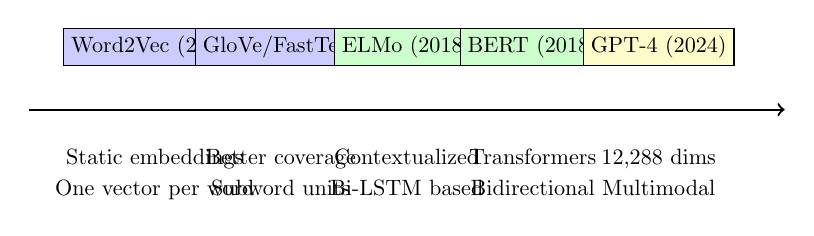
\begin{tikzpicture}[scale=0.8, transform shape]
        % Timeline arrow
        \draw[thick,->] (0,0) -- (12,0);
        
        % Word2Vec era
        \node[draw, fill=blue!20] at (2,1) {Word2Vec (2013)};
        \node[below] at (2,-0.5) {Static embeddings};
        \node[below] at (2,-1) {One vector per word};
        
        % GloVe/FastText
        \node[draw, fill=blue!20] at (4,1) {GloVe/FastText};
        \node[below] at (4,-0.5) {Better coverage};
        \node[below] at (4,-1) {Subword units};
        
        % ELMo
        \node[draw, fill=green!20] at (6,1) {ELMo (2018)};
        \node[below] at (6,-0.5) {Contextualized};
        \node[below] at (6,-1) {Bi-LSTM based};
        
        % BERT
        \node[draw, fill=green!20] at (8,1) {BERT (2018)};
        \node[below] at (8,-0.5) {Transformers};
        \node[below] at (8,-1) {Bidirectional};
        
        % GPT
        \node[draw, fill=yellow!20] at (10,1) {GPT-4 (2024)};
        \node[below] at (10,-0.5) {12,288 dims};
        \node[below] at (10,-1) {Multimodal};
    \end{tikzpicture}
    
    \vspace{1em}
    \textbf{Key Progression:}
    \begin{itemize}
        \item Static → Contextualized
        \item Words → Subwords → Tokens
        \item 300 dims → 12,288 dims
        \item Single task → Multi-task → General intelligence
    \end{itemize}
\end{frame}


% Future Directions
\begin{frame}[t]{Future Directions: What's Next?}
    \textbf{Current Research (2024):}
    \begin{itemize}
        \item \textbf{Efficient Embeddings:} Maintain quality at 64 dimensions
        \item \textbf{Multimodal:} Text + Image + Audio in same space
        \item \textbf{Dynamic:} Embeddings that update with new information
        \item \textbf{Personalized:} User-specific embedding spaces
    \end{itemize}
    
    \vspace{0.5em}
    \textbf{Challenges Being Solved:}
    \begin{itemize}
        \item \textbf{Long Context:} Embed entire books (1M+ tokens)
        \item \textbf{Cross-lingual:} Universal embeddings for all languages
        \item \textbf{Interpretability:} Understanding what each dimension means
        \item \textbf{Continual Learning:} Updating without forgetting
    \end{itemize}
    
    \vspace{0.5em}
    \textbf{Connection to Next Week:}
    \begin{itemize}
        \item Week 3: RNNs - Processing sequences with embeddings
        \item Embeddings are the input to all modern NLP models
        \item Foundation we'll build on for rest of course
    \end{itemize}
\end{frame}

% Course Summary
\begin{frame}[t]{Week 2 Summary: Words Have Meaning!}
    \textbf{Journey We Took:}
    \begin{enumerate}
        \item Started with words as meaningless IDs
        \item Learned the distributional hypothesis
        \item Built Word2Vec from scratch
        \item Tackled challenges (scale, bias, polysemy)
        \item Applied to real problems
    \end{enumerate}
    
    \vspace{0.5em}
    \textbf{Key Takeaways:}
    \begin{itemize}
        \item \highlight{Core Insight:} Similar contexts → Similar meanings
        \item \highlight{Technical:} Skip-gram + negative sampling = efficient training
        \item \highlight{Practical:} Embeddings power all modern AI
        \item \highlight{Evolution:} Static → Contextualized → Multimodal
    \end{itemize}
    
    \vspace{0.5em}
    \textbf{Your Homework:}
    \begin{itemize}
        \item Build semantic search engine (notebook provided)
        \item Explore biases in pre-trained embeddings
        \item Try word arithmetic with different models
    \end{itemize}
    
    \vspace{0.5em}
    \begin{center}
        \colorbox{green!20}{
            \parbox{0.8\textwidth}{
                \centering
                \textbf{Remember:} Every ChatGPT response starts with embeddings!
            }
        }
    \end{center}
\end{frame}


\begin{frame}[t]{Neural LM Era (2003-2013): Learning Representations}
    \textbf{Bengio's breakthrough: Learn while predicting}
    
    \vspace{0.5em}
    \begin{columns}[T]
        \begin{column}{0.5\textwidth}
            \textbf{Vocabulary:}
            \begin{itemize}
                \item Larger fixed vocabulary (50k)
                \item Learned word embeddings (30-100 dim)
                \item Still word-level tokenization
            \end{itemize}
            
            \vspace{0.5em}
            \textbf{Context:}
            \begin{itemize}
                \item Fixed window with hidden states
                \item Concatenate embedding vectors
                \item Some semantic understanding
            \end{itemize}
            
            \vspace{0.5em}
            \textbf{Key Innovations:}
            \begin{itemize}
                \item \highlight{Distributed representations}
                \item \highlight{End-to-end learning}
                \item \highlight{Generalization beyond seen n-grams}
            \end{itemize}
        \end{column}
        \begin{column}{0.5\textwidth}
            \textbf{Architecture (Bengio 2003):}
            \begin{enumerate}
                \item Input: Previous n-1 words
                \item Lookup: Word → Embedding vector
                \item Concatenate: $[e_{w_{t-2}}, e_{w_{t-1}}]$
                \item Hidden layer: $h = \tanh(H \cdot x + b)$
                \item Output: $y = \text{softmax}(W \cdot h)$
            \end{enumerate}
            
            \vspace{0.5em}
            \textbf{Training:}
            \begin{itemize}
                \item Minimize cross-entropy loss
                \item Backpropagation through time
                \item Learn embeddings + weights jointly
            \end{itemize}
            
            \vspace{0.5em}
            \textbf{Computational Cost:}
            \begin{itemize}
                \item Training: Days to weeks
                \item Inference: $O(|V| \cdot H)$ per word
            \end{itemize}
        \end{column}
    \end{columns}
    
    \vspace{0.3em}
    \highlight{Impact:} 30-50\% perplexity reduction vs n-grams + Similar words get similar embeddings!
\end{frame}

\begin{frame}[t]{Embedding Era (2013-2017): Semantic Understanding}
    \textbf{Word2Vec/GloVe: Meaning before prediction}
    
    \vspace{0.5em}
    \begin{columns}[T]
        \begin{column}{0.5\textwidth}
            \textbf{Vocabulary:}
            \begin{itemize}
                \item Large vocabularies (100k-1M)
                \item Rich 100-300 dim embeddings
                \item Subword models (FastText)
            \end{itemize}
            
            \vspace{0.5em}
            \textbf{Context:}
            \begin{itemize}
                \item Window-based but semantic
                \item Skip-gram: predict context from center
                \item CBOW: predict center from context
            \end{itemize}
        \end{column}
        \begin{column}{0.5\textwidth}
            \textbf{Method:}
            \begin{itemize}
                \item Separate embedding training
                \item Negative sampling for efficiency
                \item Cosine similarity for prediction
            \end{itemize}
            
            \vspace{0.5em}
            \textbf{Next-word prediction:}
            $$P(w_{next}|context) \propto \exp(v_{context}^T \cdot v_{w_{next}})$$
            
            Find: $\argmax_w \cos(v_w, v_{context})$
        \end{column}
    \end{columns}
    
    \vspace{0.5em}
    \centering
    \includegraphics[width=0.8\textwidth]{../figures/week2_embedding_space.pdf}
\end{frame}

\begin{frame}[t]{Transformer Era (2017-Present): Attention is All You Need}
    \textbf{BERT, GPT: Context-aware predictions}
    
    \vspace{0.5em}
    \begin{columns}[T]
        \begin{column}{0.5\textwidth}
            \textbf{Vocabulary:}
            \begin{itemize}
                \item Subword tokens (30k-50k BPE/WordPiece)
                \item No OOV problem
                \item Multilingual support
            \end{itemize}
            
            \vspace{0.5em}
            \textbf{Context:}
            \begin{itemize}
                \item Full sequence (512-32k+ tokens)
                \item Bidirectional (BERT) or causal (GPT)
                \item Positional encodings
            \end{itemize}
        \end{column}
        \begin{column}{0.5\textwidth}
            \textbf{Method:}
            \begin{itemize}
                \item Self-attention mechanism
                \item Multi-head attention
                \item Deep architectures (12-96+ layers)
            \end{itemize}
            
            \vspace{0.5em}
            \textbf{Prediction:}
            $$\text{Attention}(Q,K,V) = \text{softmax}\left(\frac{QK^T}{\sqrt{d_k}}\right)V$$
            
            Context-dependent embeddings!
        \end{column}
    \end{columns}
    
    \vspace{0.5em}
    \textbf{Revolutionary Features:}
    \begin{itemize}
        \item "King" has different embeddings in "King of England" vs "King bed"
        \item Can handle: "The \_\_\_ that I saw yesterday was \_\_\_" (long-range)
        \item Zero-shot learning capabilities
    \end{itemize}
\end{frame}

\begin{frame}[t]{Comparing Prediction Approaches: Same Task, Different Methods}
    \textbf{Task:} Predict next word after "The cat sat on the \_\_\_"
    
    \vspace{0.5em}
    \begin{center}
    \small
    \begin{tabular}{|l|p{3.5cm}|p{3.5cm}|p{3.5cm}|}
        \hline
        \textbf{Era} & \textbf{How it Works} & \textbf{Top Predictions} & \textbf{Why?} \\
        \hline
        \hline
        \textbf{N-grams} & Count "cat sat on the X" in corpus & mat (0.6), floor (0.2), chair (0.1) & Pure statistics \\
        \hline
        \textbf{Neural LM} & Learned patterns from embeddings & mat (0.4), floor (0.3), carpet (0.2) & Semantic similarity \\
        \hline
        \textbf{Word2Vec} & Find words similar to context vector & mat (0.35), rug (0.25), surface (0.20) & Geometric proximity \\
        \hline
        \textbf{GPT-4} & Attention over entire context & mat (0.3), [depends on prior context] & Full understanding \\
        \hline
    \end{tabular}
    \end{center}
    
    \vspace{0.5em}
    \textbf{Key Evolution:}
    \begin{itemize}
        \item \textbf{N-grams:} What words followed this sequence before?
        \item \textbf{Neural/Embeddings:} What words are semantically appropriate?
        \item \textbf{Transformers:} What makes sense given everything?
    \end{itemize}
\end{frame}


%============================================================================
\section{Appendix A: Mathematical Foundations}
%============================================================================

\begin{frame}[t]{Appendix A: Skip-gram Objective Derivation}
    \textbf{Full Mathematical Formulation:}
    
    Given a sequence of words $w_1, w_2, ..., w_T$, maximize:
    $$\mathcal{L} = \frac{1}{T} \sum_{t=1}^{T} \sum_{-c \leq j \leq c, j \neq 0} \log P(w_{t+j} | w_t)$$
    
    Where:
    $$P(w_O | w_I) = \frac{\exp(v_{w_O}^{'T} v_{w_I})}{\sum_{w=1}^{W} \exp(v_w^{'T} v_{w_I})}$$
    
    \vspace{0.5em}
    \textbf{Gradient with respect to center word:}
    $$\frac{\partial \log P(w_O | w_I)}{\partial v_{w_I}} = v_{w_O}' - \sum_{w=1}^{W} P(w|w_I) \cdot v_w'$$
    
    \vspace{0.5em}
    \textbf{Interpretation:}
    \begin{itemize}
        \item First term: Move toward actual context word
        \item Second term: Move away from expected context (all words weighted by probability)
        \item Result: Embeddings organize by co-occurrence patterns
    \end{itemize}
\end{frame}

\begin{frame}[t]{Appendix A: Negative Sampling Mathematics}
    \textbf{Original objective (expensive):}
    $$\log P(w_O | w_I) = \log \frac{\exp(v_{w_O}^{'T} v_{w_I})}{\sum_{w=1}^{W} \exp(v_w^{'T} v_{w_I})}$$
    
    \textbf{Negative sampling objective (efficient):}
    $$\log \sigma(v_{w_O}^{'T} v_{w_I}) + \sum_{i=1}^{k} \mathbb{E}_{w_i \sim P_n(w)} [\log \sigma(-v_{w_i}^{'T} v_{w_I})]$$
    
    Where:
    \begin{itemize}
        \item $\sigma(x) = \frac{1}{1 + e^{-x}}$ (sigmoid function)
        \item $k$ = number of negative samples (typically 5-20)
        \item $P_n(w) \propto f(w)^{3/4}$ (noise distribution)
    \end{itemize}
    
    \vspace{0.5em}
    \textbf{Why it works:}
    \begin{itemize}
        \item Transforms problem to binary classification
        \item Distinguishing real from noise is sufficient
        \item Dramatically reduces computation: O(k) instead of O(W)
    \end{itemize}
\end{frame}

% New concrete example slides
\begin{frame}[t]{Concrete Example: Computing P(cat|context)}
    \textbf{Given:} "The \underline{cat} sat on the mat" with window=1
    
    \vspace{0.5em}
    \textbf{Simplified vocabulary:} \{the, cat, sat, on, mat\} = \{0, 1, 2, 3, 4\}
    
    \vspace{0.5em}
    \textbf{Embeddings (2D for visualization):}
    \begin{center}
    \begin{tabular}{|l|c|c|}
        \hline
        Word & $v$ (input) & $v'$ (output) \\
        \hline
        the & [0.5, 0.3] & [0.4, 0.6] \\
        cat & [0.8, 0.2] & [0.7, 0.4] \\
        sat & [0.3, 0.7] & [0.5, 0.8] \\
        on & [0.4, 0.5] & [0.3, 0.6] \\
        mat & [0.6, 0.4] & [0.8, 0.3] \\
        \hline
    \end{tabular}
    \end{center}
    
    \textbf{Calculate P(sat|cat):}
    \begin{align}
        v_{cat}^T \cdot v'_{sat} &= [0.8, 0.2] \cdot [0.5, 0.8] = 0.4 + 0.16 = 0.56 \\
        \exp(0.56) &= 1.75 \\
        Z &= \sum_{w} \exp(v_{cat}^T \cdot v'_w) = 1.73 + 1.75 + 1.61 + 1.87 + 1.94 = 8.9 \\
        P(sat|cat) &= \frac{1.75}{8.9} = 0.197 \approx 19.7\%
    \end{align}
\end{frame}

\begin{frame}[t]{Concrete Example: Gradient Update}
    \textbf{One gradient step for center word "cat":}
    
    \vspace{0.5em}
    \textbf{Initial:} $v_{cat} = [0.8, 0.2]$, learning rate $\alpha = 0.1$
    
    \vspace{0.5em}
    \textbf{Gradient components:}
    \begin{itemize}
        \item Positive: Pull toward "sat" (actual context)
        \item Negative: Push away from expected distribution
    \end{itemize}
    
    \vspace{0.5em}
    \textbf{Calculation:}
    \begin{align}
        \nabla &= v'_{sat} - \sum_{w} P(w|cat) \cdot v'_w \\
        &= [0.5, 0.8] - (0.194 \cdot [0.4, 0.6] + 0.197 \cdot [0.5, 0.8] + ...) \\
        &= [0.5, 0.8] - [0.48, 0.62] \\
        &= [0.02, 0.18]
    \end{align}
    
    \textbf{Update:}
    $$v_{cat}^{new} = v_{cat} + \alpha \cdot \nabla = [0.8, 0.2] + 0.1 \cdot [0.02, 0.18] = [0.802, 0.218]$$
    
    \highlight{Result: "cat" moves slightly closer to "sat" in embedding space!}
\end{frame}

\begin{frame}[t]{Concrete Example: Negative Sampling Calculation}
    \textbf{Training instance:} Center="cat", Positive="sat", Negatives=\{the, mat\}
    
    \vspace{0.5em}
    \textbf{Loss calculation step-by-step:}
    
    \vspace{0.3em}
    \textbf{1. Positive pair (cat, sat):}
    \begin{align}
        \text{score}_{pos} &= v_{cat}^T \cdot v'_{sat} = 0.56 \\
        \text{loss}_{pos} &= -\log \sigma(0.56) = -\log(0.636) = 0.452
    \end{align}
    
    \textbf{2. Negative pairs:}
    \begin{align}
        \text{score}_{neg1} &= v_{cat}^T \cdot v'_{the} = 0.52 \\
        \text{loss}_{neg1} &= -\log \sigma(-0.52) = -\log(0.373) = 0.987 \\
        \text{score}_{neg2} &= v_{cat}^T \cdot v'_{mat} = 0.70 \\
        \text{loss}_{neg2} &= -\log \sigma(-0.70) = -\log(0.332) = 1.103
    \end{align}
    
    \textbf{3. Total loss:}
    $$\text{Loss} = \text{loss}_{pos} + \text{loss}_{neg1} + \text{loss}_{neg2} = 0.452 + 0.987 + 1.103 = 2.542$$
    
    \highlight{Much faster: Only 3 calculations instead of 5,000!}
\end{frame}

\begin{frame}[t]{Concrete Example: Cosine Similarity Step-by-Step}
    \textbf{Question:} How similar are "king" and "queen"?
    
    \vspace{0.5em}
    \textbf{Given embeddings (3D for simplicity):}
    \begin{itemize}
        \item $v_{king} = [0.6, 0.8, 0.2]$
        \item $v_{queen} = [0.5, 0.7, 0.4]$
    \end{itemize}
    
    \vspace{0.5em}
    \textbf{Step 1: Calculate dot product}
    $$v_{king} \cdot v_{queen} = (0.6 \times 0.5) + (0.8 \times 0.7) + (0.2 \times 0.4) = 0.3 + 0.56 + 0.08 = 0.94$$
    
    \textbf{Step 2: Calculate magnitudes}
    \begin{align}
        ||v_{king}|| &= \sqrt{0.6^2 + 0.8^2 + 0.2^2} = \sqrt{0.36 + 0.64 + 0.04} = 1.02 \\
        ||v_{queen}|| &= \sqrt{0.5^2 + 0.7^2 + 0.4^2} = \sqrt{0.25 + 0.49 + 0.16} = 0.95
    \end{align}
    
    \textbf{Step 3: Compute cosine similarity}
    $$\cos(\theta) = \frac{v_{king} \cdot v_{queen}}{||v_{king}|| \times ||v_{queen}||} = \frac{0.94}{1.02 \times 0.95} = \frac{0.94}{0.969} = 0.97$$
    
    \highlight{Interpretation: 0.97 = Very similar! (1.0 = identical, 0 = orthogonal)}
\end{frame}

% Enhanced Mathematical Appendix
\begin{frame}[t]{Appendix A: CBOW Objective Function}
    \textbf{Continuous Bag-of-Words (CBOW) Model:}
    
    Given context words $c = \{w_{t-m}, ..., w_{t-1}, w_{t+1}, ..., w_{t+m}\}$, predict center word $w_t$
    
    \vspace{0.5em}
    \textbf{Objective Function:}
    $$\mathcal{L} = -\frac{1}{T} \sum_{t=1}^{T} \log P(w_t | c)$$
    
    Where:
    $$P(w_t | c) = \frac{\exp(v_{w_t}^{'T} \bar{v})}{\sum_{w=1}^{W} \exp(v_w^{'T} \bar{v})}$$
    
    And $\bar{v} = \frac{1}{2m} \sum_{-m \leq j \leq m, j \neq 0} v_{w_{t+j}}$ (average of context vectors)
    
    \vspace{0.5em}
    \textbf{Gradient with respect to output embeddings:}
    $$\frac{\partial \mathcal{L}}{\partial v'_{w_t}} = \bar{v} - \sum_{w=1}^{W} P(w|c) \cdot \bar{v} = \bar{v}(1 - P(w_t|c))$$
    
    \textbf{Key Insight:} CBOW averages context to predict center (many-to-one)
\end{frame}

\begin{frame}[t]{Appendix A: GloVe Co-occurrence Matrix}
    \textbf{Global Vectors (GloVe) Formulation:}
    
    Build co-occurrence matrix $X$ where $X_{ij}$ = number of times word $j$ appears in context of word $i$
    
    \vspace{0.5em}
    \textbf{Objective Function:}
    $$J = \sum_{i,j=1}^{V} f(X_{ij})(w_i^T \tilde{w}_j + b_i + \tilde{b}_j - \log X_{ij})^2$$
    
    Where weighting function:
    $$f(x) = \begin{cases}
        (x/x_{max})^{\alpha} & \text{if } x < x_{max} \\
        1 & \text{otherwise}
    \end{cases}$$
    
    Typically: $x_{max} = 100$, $\alpha = 0.75$
    
    \vspace{0.5em}
    \textbf{Key Insights:}
    \begin{itemize}
        \item Combines global statistics (co-occurrence) with local context
        \item Directly encodes semantic relationships: $w_i^T w_j \approx \log P(j|i)$
        \item Training on co-occurrence ratios captures meaning
    \end{itemize}
\end{frame}

\begin{frame}[t]{Appendix A: Subsampling Frequent Words}
    \textbf{Problem:} Frequent words like "the", "a" provide less information
    
    \vspace{0.5em}
    \textbf{Subsampling Probability:}
    
    For word $w_i$ with frequency $f(w_i)$, discard with probability:
    $$P(\text{discard } w_i) = 1 - \sqrt{\frac{t}{f(w_i)}}$$
    
    Where $t$ is threshold (typically $10^{-5}$)
    
    \vspace{0.5em}
    \textbf{Example with actual frequencies:}
    \begin{center}
    \begin{tabular}{|l|c|c|c|}
        \hline
        Word & Frequency & P(keep) & Effect \\
        \hline
        "the" & 0.07 & 0.038 & Keep 3.8\% \\
        "computer" & 0.0001 & 1.0 & Keep 100\% \\
        "neural" & 0.00005 & 1.0 & Keep 100\% \\
        \hline
    \end{tabular}
    \end{center}
    
    \textbf{Impact:}
    \begin{itemize}
        \item Speeds up training by 2-10x
        \item Improves quality of rare word vectors
        \item Balances the training signal
    \end{itemize}
\end{frame}

\begin{frame}[t]{Appendix A: t-SNE for Embedding Visualization}
    \textbf{t-Distributed Stochastic Neighbor Embedding:}
    
    Reduce high-dimensional embeddings to 2D/3D for visualization
    
    \vspace{0.5em}
    \textbf{High-dimensional similarity (Gaussian):}
    $$p_{j|i} = \frac{\exp(-||x_i - x_j||^2 / 2\sigma_i^2)}{\sum_{k \neq i} \exp(-||x_i - x_k||^2 / 2\sigma_i^2)}$$
    
    \textbf{Low-dimensional similarity (Student-t):}
    $$q_{ij} = \frac{(1 + ||y_i - y_j||^2)^{-1}}{\sum_{k \neq l} (1 + ||y_k - y_l||^2)^{-1}}$$
    
    \textbf{Minimize KL divergence:}
    $$C = \sum_i KL(P_i || Q_i) = \sum_i \sum_j p_{ij} \log \frac{p_{ij}}{q_{ij}}$$
    
    \vspace{0.5em}
    \textbf{Gradient:}
    $$\frac{\partial C}{\partial y_i} = 4 \sum_j (p_{ij} - q_{ij})(y_i - y_j)(1 + ||y_i - y_j||^2)^{-1}$$
    
    \textbf{Result:} Preserves local structure while revealing global patterns
\end{frame}


%============================================================================
\section{Appendix C: Extended Examples}
%============================================================================

\begin{frame}[t]{Appendix C: Domain-Specific Embeddings}
    \textbf{Medical Embeddings (BioWordVec):}
    \begin{itemize}
        \item Trained on PubMed + MIMIC-III
        \item Captures: drug-disease relationships
        \item Application: Clinical decision support
    \end{itemize}
    
    \textbf{Legal Embeddings (Law2Vec):}
    \begin{itemize}
        \item Trained on case law + statutes
        \item Captures: Legal concept similarity
        \item Application: Legal document search
    \end{itemize}
    
    \textbf{Financial Embeddings (FinBERT):}
    \begin{itemize}
        \item Trained on financial news + reports
        \item Captures: Market sentiment
        \item Application: Trading signals
    \end{itemize}
    
    \textbf{Code Embeddings (CodeBERT):}
    \begin{itemize}
        \item Trained on GitHub repositories
        \item Captures: Programming patterns
        \item Application: Code search, bug detection
    \end{itemize}
    
    \vspace{0.5em}
    \highlight{Lesson: Domain-specific training dramatically improves performance}
\end{frame}

% Final slide
\begin{frame}[t]{References and Resources}
    \textbf{Essential Papers:}
    \begin{itemize}
        \item Mikolov et al. (2013). "Efficient estimation of word representations in vector space"
        \item Mikolov et al. (2013). "Distributed representations of words and phrases"
        \item Pennington et al. (2014). "GloVe: Global vectors for word representation"
        \item Peters et al. (2018). "Deep contextualized word representations" (ELMo)
    \end{itemize}
    
    \textbf{Implementations:}
    \begin{itemize}
        \item Gensim: \url{https://radimrehurek.com/gensim/}
        \item FastText: \url{https://fasttext.cc/}
        \item Hugging Face: \url{https://huggingface.co/}
    \end{itemize}
    
    \textbf{Datasets:}
    \begin{itemize}
        \item Google Analogy Test Set
        \item WordSim-353
        \item SimLex-999
    \end{itemize}
    
    \textbf{Next Week:} Recurrent Neural Networks - Processing sequences with embeddings
\end{frame}

\end{document}